% This file was created with tikzplotlib v0.10.1.
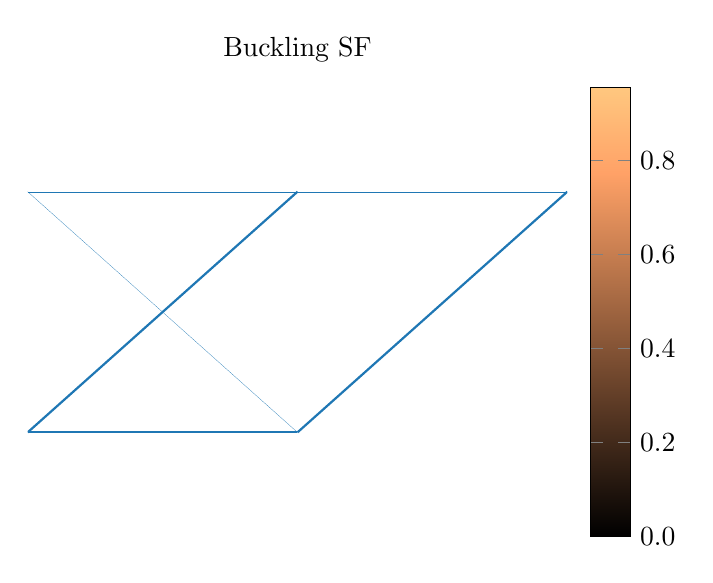
\begin{tikzpicture}

\definecolor{darkgray176}{RGB}{176,176,176}
\definecolor{steelblue31119180}{RGB}{31,119,180}

\begin{axis}[
colorbar,
colorbar style={ytick={0,0.2,0.4,0.6,0.8,1},yticklabels={
  \(\displaystyle {0.0}\),
  \(\displaystyle {0.2}\),
  \(\displaystyle {0.4}\),
  \(\displaystyle {0.6}\),
  \(\displaystyle {0.8}\),
  \(\displaystyle {1.0}\)
},ylabel={}},
colormap={mymap}{[1pt]
  rgb(0pt)=(0,0,0);
  rgb(17pt)=(1,0.6324001488,0.40273819);
  rgb(21pt)=(1,0.7812,0.4975)
},
hide x axis,
hide y axis,
point meta max=0.954929659301962,
point meta min=0,
tick align=outside,
tick pos=left,
title={Buckling SF},
x grid style={darkgray176},
xmin=0, xmax=720,
xtick style={color=black},
y grid style={darkgray176},
ymin=-155.322580645161, ymax=515.322580645161,
ytick style={color=black}
]
\path [draw=steelblue31119180, line width=0.117100818266922pt]
(axis cs:0,360)
--(axis cs:360,360);

\path [draw=steelblue31119180, line width=0.0585504089669642pt]
(axis cs:360,360)
--(axis cs:720,360);

\path [draw=steelblue31119180, line width=0.672717132193106pt]
(axis cs:0,0)
--(axis cs:360,0);

\path [draw=steelblue31119180, line width=0.0828027825326282pt]
(axis cs:360,0)
--(axis cs:0,360);

\path [draw=steelblue31119180, thick]
(axis cs:0,0)
--(axis cs:360,360);

\path [draw=steelblue31119180, line width=0.799999999631368pt]
(axis cs:360,0)
--(axis cs:720,360);

\end{axis}

\end{tikzpicture}
